\documentclass[11pt,a4paper]{article}

\usepackage[margin=2.4cm]{geometry}
\usepackage[T1]{fontenc}
\usepackage[utf8]{inputenc}
\usepackage{lmodern}
\usepackage{booktabs}
\usepackage{tabularx}
\usepackage{array}
\usepackage{graphicx}
\usepackage{float}
\usepackage{listings}
\usepackage{hyperref}
\usepackage{xcolor}

\hypersetup{colorlinks=true,linkcolor=black,urlcolor=blue!50!black}

\lstset{
  basicstyle=\ttfamily\small,
  breaklines=true,
  columns=fullflexible,
  frame=single,
  framerule=0.3pt,
  backgroundcolor=\color{gray!8}
}

\title{I05 report: 8-bit CORDIC sine and cosine\\
\large Version \textperiodcentered\ date}
\author{Truong Hai Minh\\Student ID 24100706}
\date{}

\begin{document}
\maketitle

% The section titles follow the teacher's package:
% 01 Requirement, 02 Specification, 03 Architecture,
% 04 Implementation, 05 Verification.
% Section 6 continues the physical flow. In that package, 06 GDSII
% is only partly filled. This report may record the completed local run.
% Section 7 is the traceability folder from the same package.
% Please write each part in your own words. The notes are only reminders.

\begin{table}[H]
  \centering
  \caption{Where each charter item may be addressed.}
  \begin{tabular}{@{}cl@{}}
    \toprule
    Charter item & Section \\
    \midrule
    Application context & Requirement \\
    System block diagram & Architecture \\
    Analog, digital, or mixed classification & Architecture \\
    Interface table & Specification \\
    Annotated digital artifact & Verification, and Physical result \\
    Lifecycle & Implementation \\
    RTM-lite & Traceability \\
    What has been shown, and what has not & Traceability \\
    \bottomrule
  \end{tabular}
\end{table}

\tableofcontents

\section{Requirement}

\subsection{Application}
Sine and cosine appear often in a digital test waveform. A direct implementation either stores a large table or multiplies wide data, and both choices spend area. This work uses CORDIC, the classical shift-and-add method of Volder (1959), so that one sample can be formed by addition, subtraction, and shifting. The extra cost is a sequence of clocks for each sample.

The block is asked to supply one sine value and one cosine value for that waveform. The user presents one unsigned angle byte, in which one step equals \(360^\circ/256\), together with one start pulse. The block returns one signed pair. It is a digital core placed behind the Tiny Tapeout pin shell. It is not a full signal generator, and it does not accumulate a phase from sample to sample. The complete analog, digital, or mixed classification is given in the Architecture section.

\subsection{Requirements}
The application above says what the block is for. The list below is what this work is asked to meet, including the boundary of the work.

\begin{itemize}
  \item An 8-bit CORDIC in rotation mode, eight steps: one unsigned angle byte and one start pulse produce one signed sine and one signed cosine.
  \item The pins are \texttt{ui\_in[7:0]} for the angle, \texttt{uio\_in[0]} for start, \texttt{uo\_out[7:0]} for sine, and \texttt{uio\_out[7:0]} for cosine.
  \item The charter angles are code 0 (\(0^\circ\)), code 21 (\(29.53^\circ\), the byte nearest \(30^\circ\)), code 32 (\(45^\circ\)), code 43 (\(60.47^\circ\), the byte nearest \(60^\circ\)), and code 64 (\(90^\circ\)).
  \item Two further angles are chosen for this design: code 96 (\(135^\circ\)) and code 255 (\(358.59^\circ\)), one step before a full turn. Code 255 is the corner.
  \item The error table uses these ten codes: 0, 21, 32, 43, 64, 96, 128 (\(180^\circ\)), 192 (\(270^\circ\)), 224 (\(315^\circ\)), and 255. Each row is compared with true sine and cosine.
  \item A cell report shows no multiply cell, and it counts the cells that hold the arctangent constants.
  \item Three questions are answered: the area compared with a multiplier, the error after eight steps, and the cell cost of the arctangent constants.
  \item The report carries a version and a date.
  \item Inside the work: the sequential core, simulation of the Tiny Tapeout pin shell, the checks above, and the OpenLane run \texttt{RUN\_2026.10.03\_09.21.28} with its GDS. The layout top is \texttt{cordic}. The shell \texttt{tt\_um\_cordic} is simulated and is not the layout top.
  \item Outside the work: vector mode, floating point, a wider output, a transistor-level analog circuit, a second layout run, a fabricated chip, tape-out, and any claim of sign-off.
\end{itemize}

\section{Specification}

The requirement names the block and the angles. This section states the contract those later checks are judged against. It begins with the behaviour, then the pins, the clocks, the fixed numbers, and the corners.

One unsigned byte is the angle. One step of that byte equals \(360^\circ/256\). A start pulse accepted in idle runs one rotation-mode CORDIC of eight steps and returns one signed sine and one signed cosine. The value 127 stands for about \(+1\), and \(-128\) stands for about \(-1\). The same eight \texttt{uio} wires carry start while the core is idle and carry cosine on the cycle \texttt{done} is high. \texttt{done} itself stays inside the core.

\subsection{Functional specification}
The core waits in idle. A high \texttt{start} in that state moves it to load and clears the step index. \texttt{angle\_fold} maps the byte into the first quadrant, so the working angle is in \(0\) to \(64\) brads, and it stores the sign of sine and the sign of cosine. The four ranges are codes \(0\)--\(63\), \(64\)--\(127\), \(128\)--\(191\), and \(192\)--\(255\).

On the load cycle the datapath sets \(x = K = 9949\), \(y = 0\), and \(z\) to the folded angle. \(K\) is the CORDIC gain, kept in 16 bits because it does not fit in eight bits. The folded angle is captured with \(z\), so a later change of the input byte does not change the quadrant of this run.

Eight run cycles follow, with the step index from 0 to 7. The direction is the sign of \(z\): a non-negative \(z\) rotates one way, and a negative \(z\) rotates the other way. Each step adds or subtracts a shifted copy of \(x\) and of \(y\), and adds or subtracts one stored arctangent step from \(z\). Those eight steps, in brads, are 32, 19, 10, 5, 3, 1, 1, and 0. The last step is 0, so it does not steer \(z\). No step multiplies.

On the sample cycle, \(x\) and \(y\) are shifted down by seven bits and clamped to \(-128\) through \(127\). The stored signs are applied. Sine and cosine are written on the next clock and then held. The state returns to idle. \texttt{done} is high for that one clock only.

\subsection{Interface}
The behaviour above uses a small set of wires. Each wire is named here with its direction, width, active level, and the assumption a reader needs before trusting a later result.

The shell is \texttt{tt\_um\_cordic}. The core inside it is \texttt{cordic}. \texttt{clk} and \texttt{rst\_n} sit beside the 24 Tiny Tapeout data pins. \texttt{ena} is present on the shell and is not used. \texttt{uio\_in[7:1]} is not used. Start is ignored while \texttt{done} is high, so cosine bit 0 cannot be read as a new start.

\begin{table}[ht]
\centering
\caption{Interface of the pin shell and the core.}
\label{tab:interface}
\begin{tabular}{lllll}
\toprule
Name & Direction & Width & Active level & Assumption \\
\midrule
\texttt{clk} & in & 1 & rising edge & one step of the state machine \\
\texttt{rst\_n} & in & 1 & low & asynchronous, on every register \\
\texttt{ui\_in[7:0]} & in & 8 & level & angle byte, valid when load captures \(z\) \\
\texttt{uio\_in[0]} & in & 1 & high & start, accepted only in idle \\
\texttt{uo\_out[7:0]} & out & 8 & signed & sine, held between samples \\
\texttt{uio\_out[7:0]} & out & 8 & signed & cosine, driven while \texttt{done} is high \\
\texttt{uio\_oe[7:0]} & out & 8 & high & \texttt{8'hff} while \texttt{done}, else \texttt{8'h00} \\
\texttt{done} & internal & 1 & high & one clock, not a shell pin \\
\bottomrule
\end{tabular}
\end{table}

\subsection{Timing}
The pins say which wire is start and which wire is the result. The clocks below say when a start is accepted and when the pair is stored. Reset is asynchronous and active-low. After reset the state is idle and the held sine and cosine are 0.

A start seen in idle is accepted on the rising clock. The next clock is the load cycle. Eight run clocks follow, and then one sample clock. \texttt{done} is registered from that sample state, so it is high for one clock after the sample state, and the new sine and cosine are in the output registers on that same clock. The core is idle again while \texttt{done} is high. A start on that clock is ignored.

The period of 10\,ns and the pin delay of 2\,ns belong to the layout run \texttt{RUN\_2026.10.03\_09.21.28}. They are constraints of that run. They are not a required clock of this block.

\subsection{Parameters}
The timing leaves the widths and the constants unnamed. They are fixed for this design as follows.

\begin{itemize}
  \item Eight iterations, rotation mode only.
  \item Angle unit: one brad is \(360^\circ/256\). The input is an unsigned byte.
  \item \(K = 9949\), the constant loaded into \(x\). In \(x\) and \(y\), the value 1.0 sits at bit 14, which is 16384. The RTL comment quotes the gain 0.607253 beside this integer. The integer itself is what the hardware loads.
  \item \(x\) and \(y\) are 16-bit signed. \(z\) and each arctangent step are 10-bit. The step index is 3 bits, and the state is 2 bits.
  \item Arctangent steps, in brads: 32, 19, 10, 5, 3, 1, 1, 0.
  \item The output shift is an arithmetic shift of seven bits, then a clamp to \(-128\) through \(127\). Full scale of the ideal comparison is 128 codes for the value 1.
\end{itemize}

\subsection{Corner cases}
The parameters are the ordinary case. The codes below are the ones that need extra care, and they are the same codes the error table will use.

The error table for this work uses ten codes: 0, 21, 32, 43, 64, 96, 128, 192, 224, and 255. Codes 21 and 43 are the bytes nearest \(30^\circ\) and \(60^\circ\). Code 96 is \(135^\circ\). Code 255 is \(358.59^\circ\), one step before a full turn, and it is the corner chosen for this design.

Code 0 still takes a first rotation, because a zero \(z\) is treated as non-negative. The last arctangent entry is 0, so step 7 does not change \(z\). The signed output is not symmetric: 127 is the positive full-scale code, and \(-128\) is the negative one. Quadrant signs are applied after the shift, so a result that lands on 0 keeps a positive code.

The measured difference from true sine and cosine is reported in Verification. It is not restated here.

\section{Architecture}

The specification is the contract. This section shows how that contract is divided into a control unit and a processing unit, and why the circuit is classified as digital.

\subsection{System diagram}
The block supplies one sample of a test waveform. A surrounding test applies one angle byte and one start pulse, waits for \texttt{done}, and reads one signed pair. Repeating that step is what draws the wave. The core does not accumulate a phase.

The simulated pin shell is \texttt{tt\_um\_cordic}. The layout top is the core \texttt{cordic}. Figure~\ref{fig:arch} shows that core in its two units.

\begin{figure}[ht]
\centering
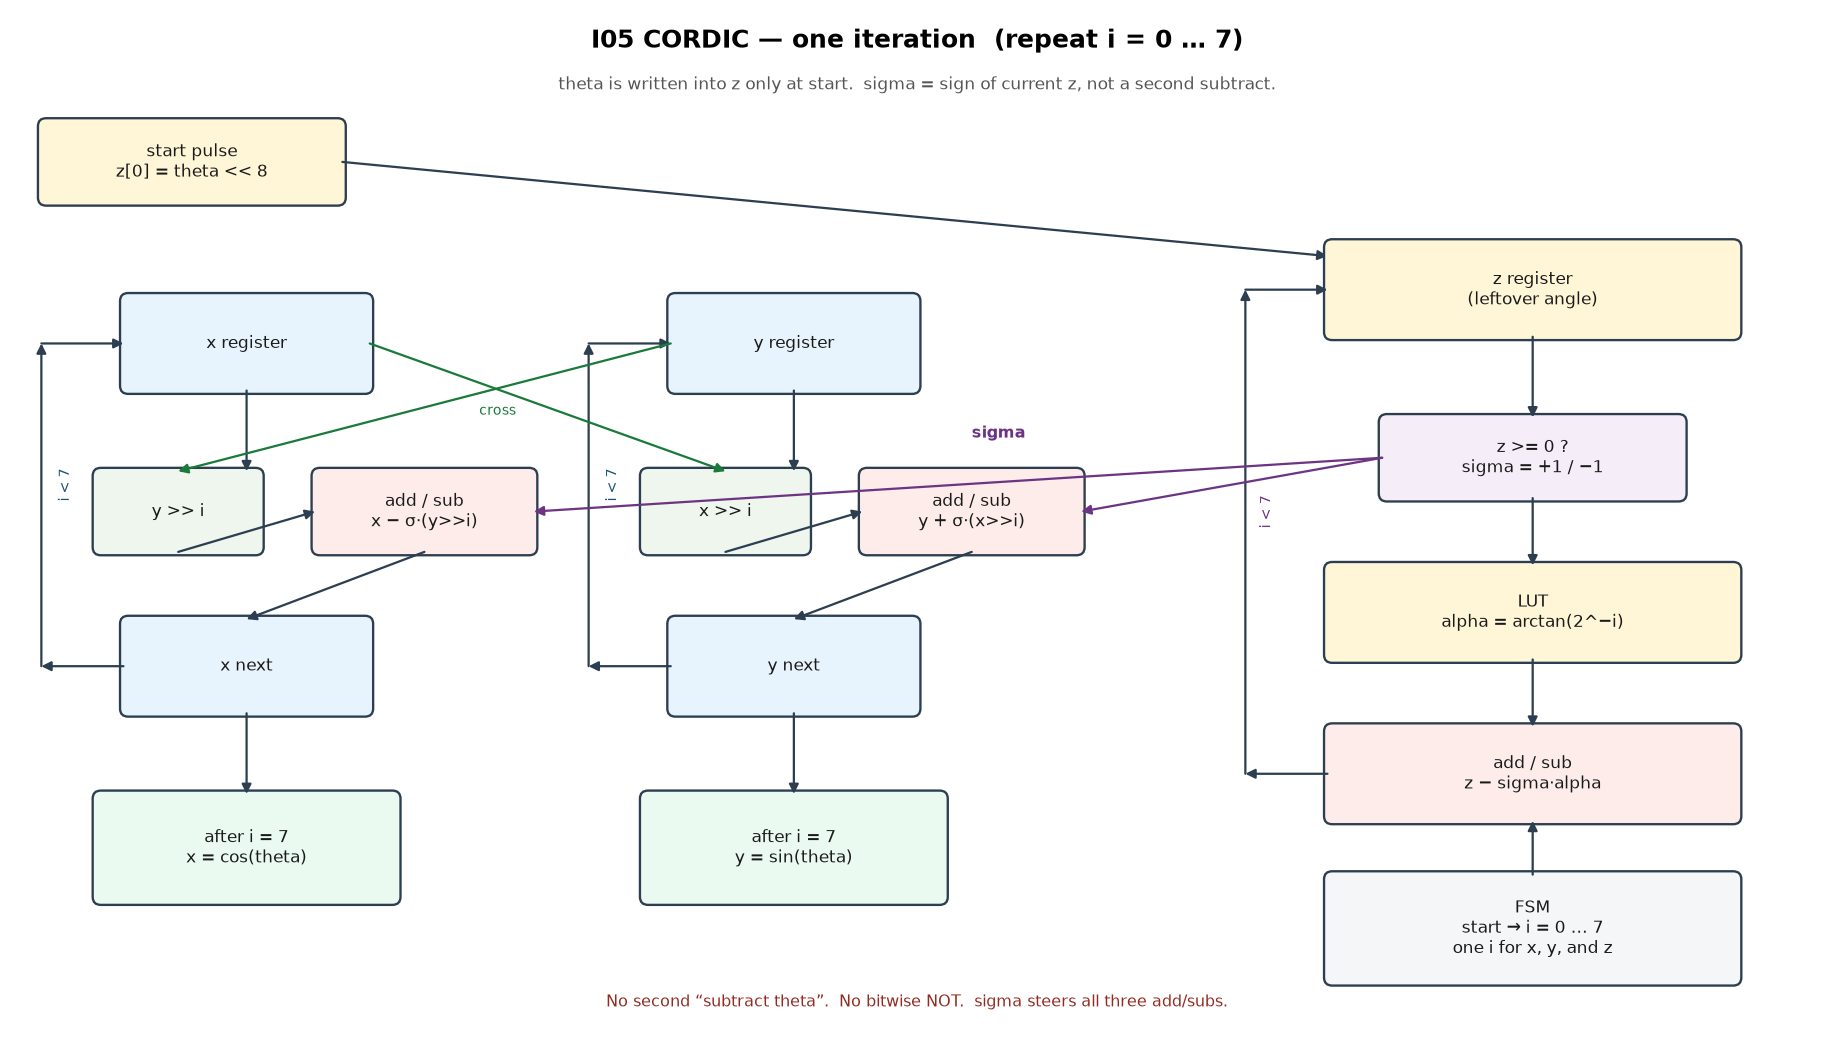
\includegraphics[width=0.85\textwidth]{architecture.png}
\caption{Core \texttt{cordic}: control beside the processing unit.}
\label{fig:arch}
\end{figure}

\subsection{Block diagram}
\texttt{cordic} wires two units.

\begin{itemize}
  \item \texttt{cordic\_control} holds the state, the step index, \texttt{done}, and the output registers. On the sample it applies \texttt{sign\_sin} and \texttt{sign\_cos}.
  \item \texttt{cordic\_processing} holds the datapath. \texttt{angle\_fold} maps the byte into \(z\) in \(0\) to \(64\) brads and produces the two signs. Block B is the 10-bit \(z\) path. Block A is the 16-bit \(x\) and \(y\) path.
\end{itemize}

\begin{figure}[ht]
\centering
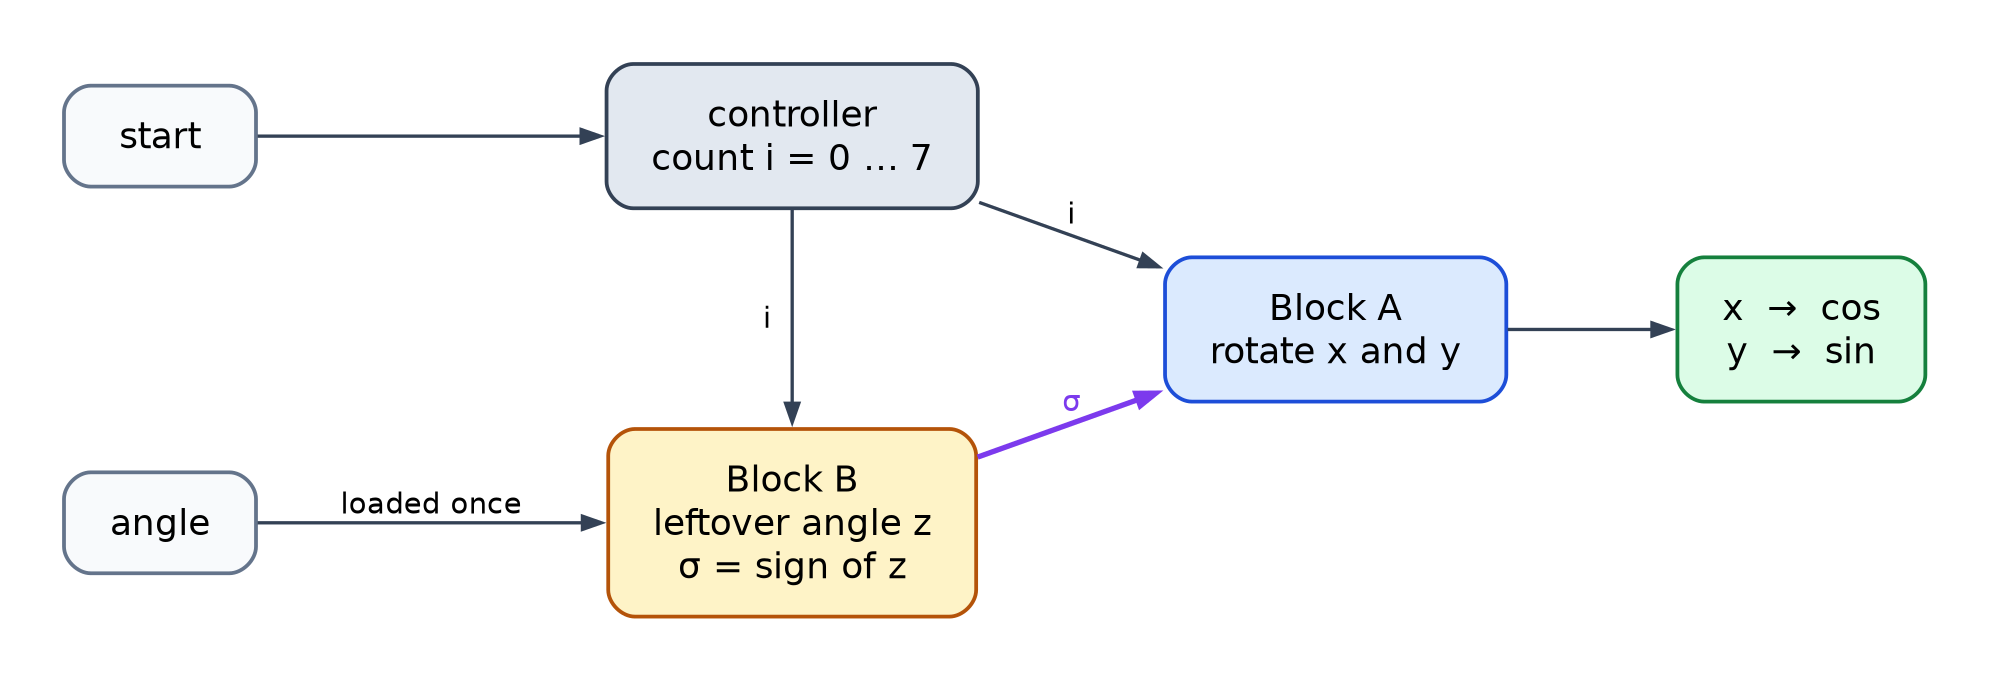
\includegraphics[width=0.85\textwidth]{block_overview.png}
\caption{Control unit and processing unit.}
\label{fig:overview}
\end{figure}

\begin{figure}[ht]
\centering
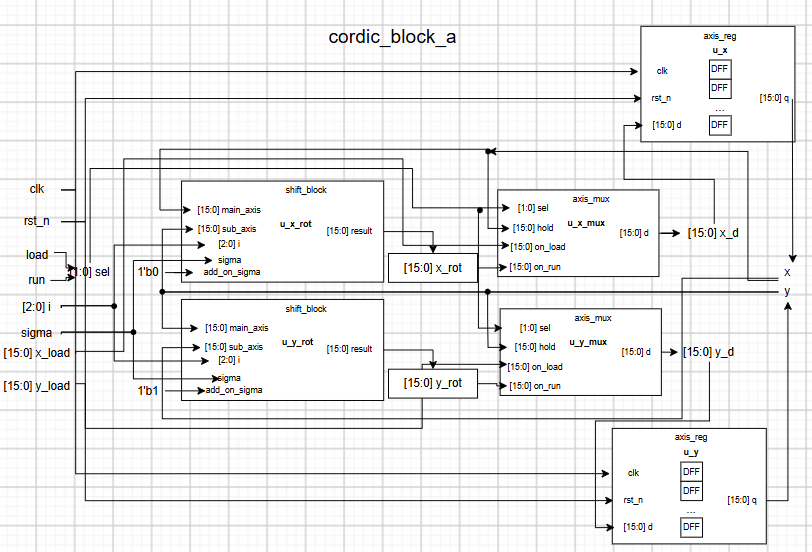
\includegraphics[width=0.48\textwidth]{structural_block_a.png}
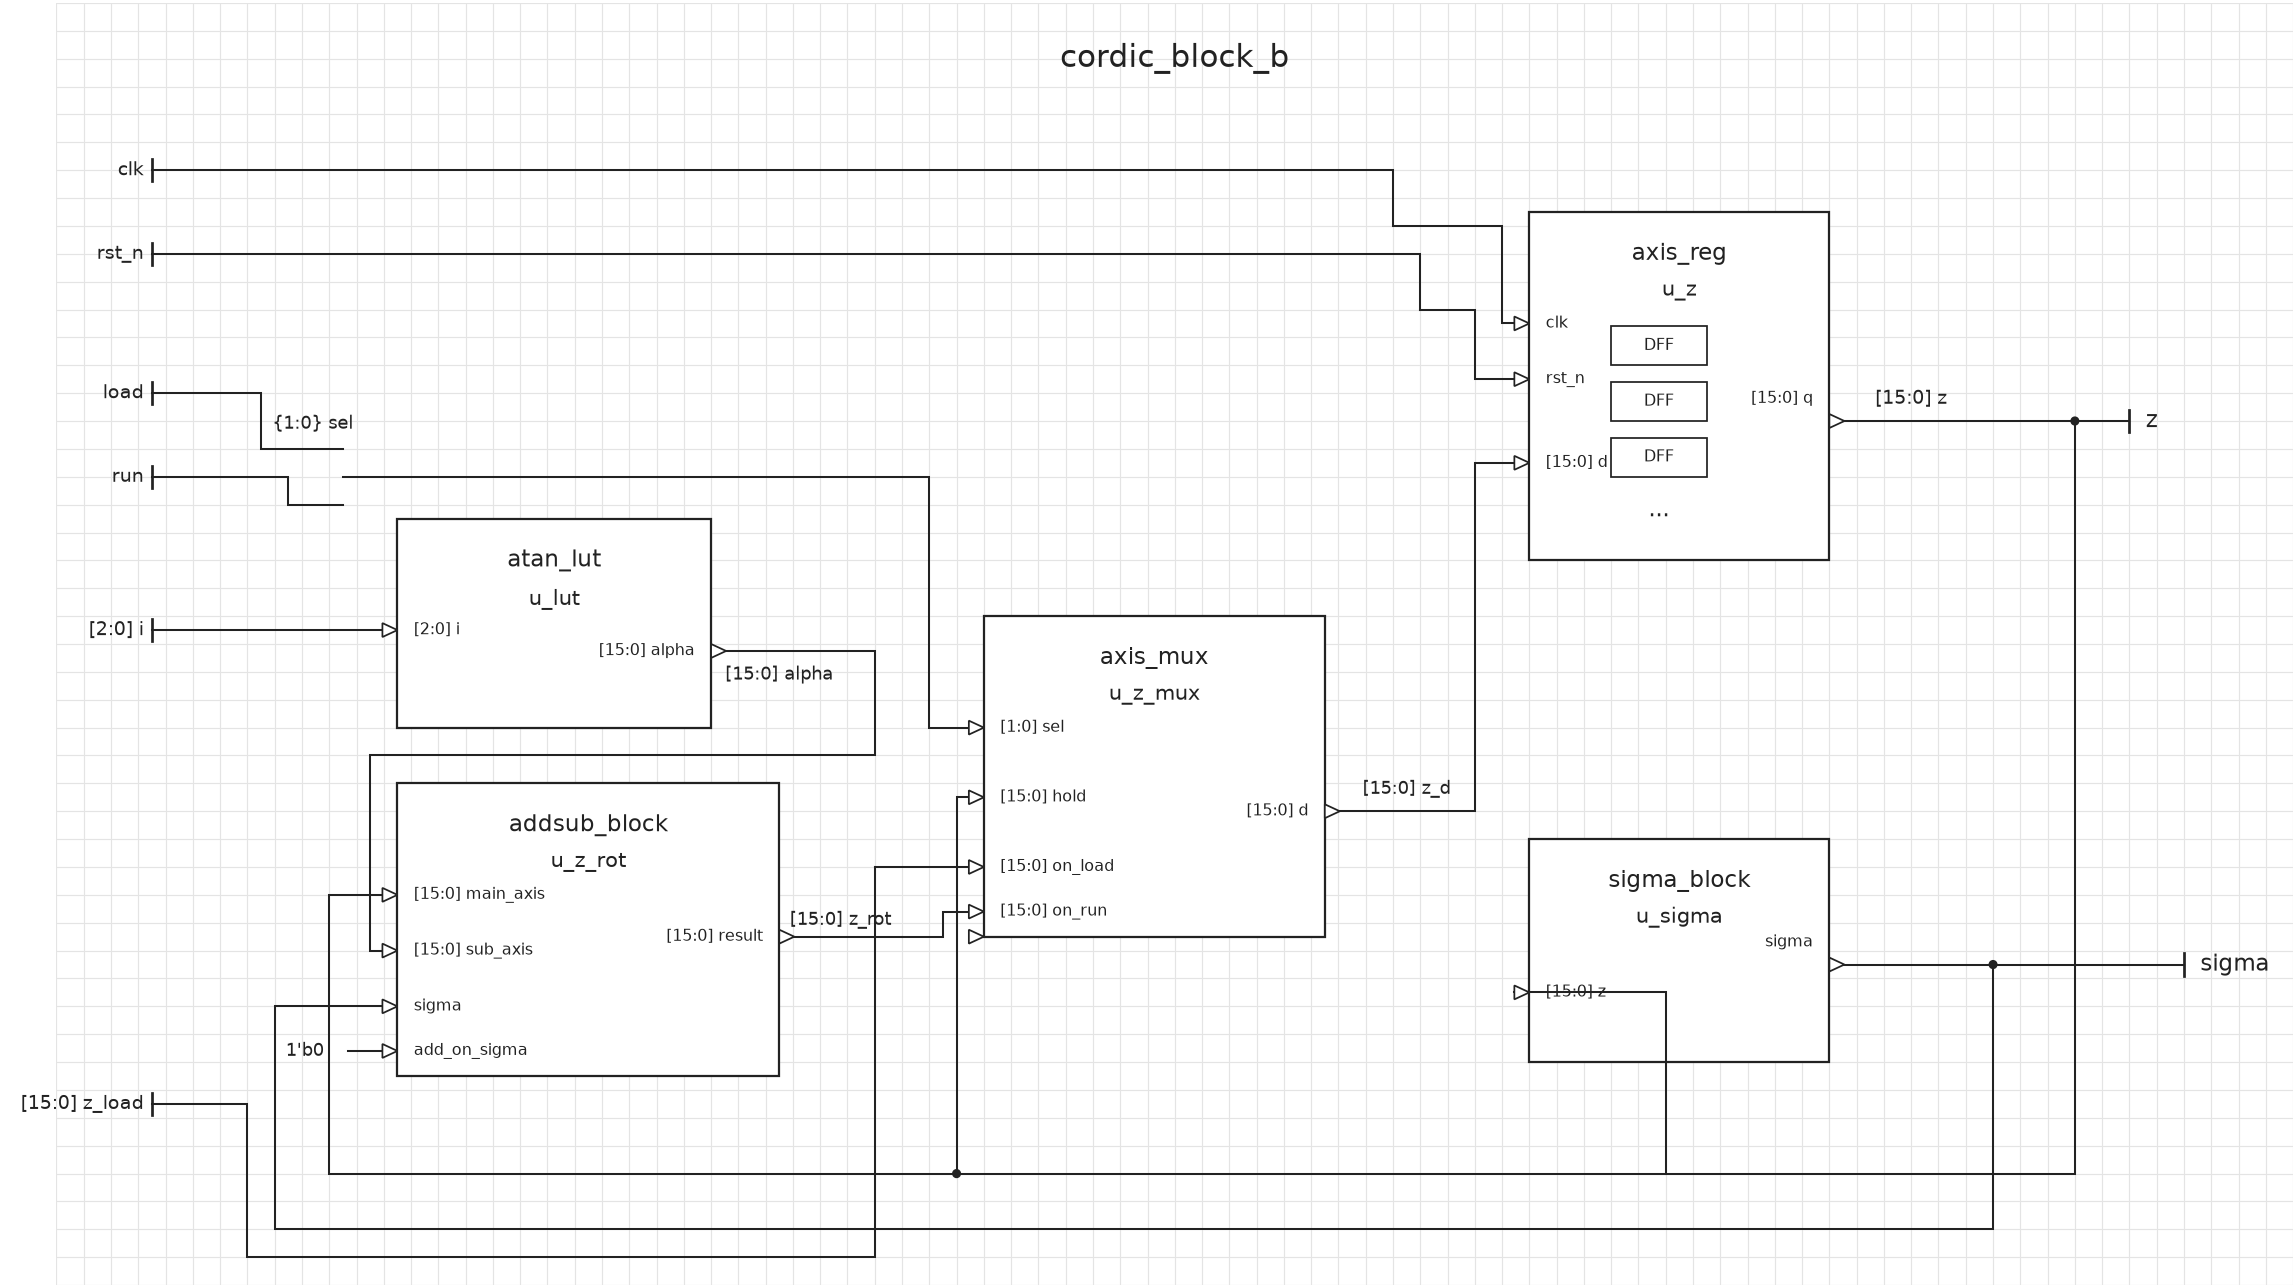
\includegraphics[width=0.48\textwidth]{structural_block_b.png}
\caption{Block A, the \(x\) and \(y\) path, and block B, the \(z\) path.}
\label{fig:ab}
\end{figure}

\subsection{Datapath}
The figures name the two units. The datapath is the processing unit, and it is the part that performs the eight steps.

Each accepted run loads \(x = 9949\), \(y = 0\), and \(z\) with the folded angle. For step \(i\), both paths add or subtract a value shifted by \(i\). The \(z\) path also adds or subtracts the arctangent constant for that step. The direction is one bit, \(\sigma = 1\) when \(z \ge 0\).

On the sample, \(x\) and \(y\) pass through \texttt{narrow\_i8}: an arithmetic shift of seven bits and a clamp to \(-128\) through \(127\). The quadrant signs then negate those bytes or leave them unchanged. The results are stored in the sine and cosine registers.

\subsection{Control}
The datapath does not decide when a step runs. The control unit does. \texttt{ctrl\_next} is combinational. Two registers hold its outputs: \texttt{u\_state} is 2 bits and \texttt{u\_i} is 3 bits. \texttt{load} is true in LOAD. \texttt{run} is true in RUN. \texttt{sample} is true in SAMPLE. \texttt{done} is a one-bit register loaded from \texttt{sample}, so it is high for one clock after the sample state.

\subsection{Finite-state machine}
Those control signals come from four states. The sequence is the behaviour already stated in the functional specification, written here as a machine.

\begin{itemize}
  \item IDLE. Wait. On \texttt{start}, go to LOAD and clear \(i\).
  \item LOAD. One clock. Capture \(x\), \(y\), \(z\), and the two signs. Go to RUN.
  \item RUN. Eight clocks, \(i\) from 0 through 7. When \(i\) is 7, go to SAMPLE.
  \item SAMPLE. One clock. Then return to IDLE.
\end{itemize}

\subsection{Timing diagram}
The state names become a clock count in Table~\ref{tab:cycles}. The count starts after the clock that accepts \texttt{start}. It is read from the state machine, not from a saved waveform log.

\begin{table}[ht]
\centering
\caption{Clocks of one accepted run.}
\label{tab:cycles}
\begin{tabular}{lll}
\toprule
Cycle & State & What is stored \\
\midrule
1 & LOAD & \(x\), \(y\), \(z\), both signs \\
2--9 & RUN & one shift-add step on each clock, \(i = 0 \ldots 7\) \\
10 & SAMPLE & narrowed sine and cosine are selected \\
11 & IDLE & sine, cosine, and \texttt{done} are written; \texttt{done} stays high this clock \\
\bottomrule
\end{tabular}
\end{table}

\subsection{Tradeoff}
The machine above spends several clocks on one sample. That choice is the tradeoff of this design. A stored table or a wide multiplier spends area on one sample. This core spends clocks instead: one load, eight iterations, and one sample. \(x\) and \(y\) are 16 bits so that \(K = 9949\) fits, which is why the flip-flop count is 66 and not the 8-bit hint of about 27 to 30. No second netlist with a multiplier was synthesized, so this report gives no percentage of area saved.

\subsection{Classification}
The tradeoff is still inside a digital circuit. The cell and register counts that support that statement are given with the classification. The circuit is digital and sequential. The sky130 netlist has 66 \texttt{sky130\_fd\_sc\_hd\_\_dfrtp\_1} cells and no memory macro. The pin shell adds no flip-flops. There is no analog block in this work.

\begin{table}[ht]
\centering
\caption{Flip-flops counted from the RTL, before the library map.}
\label{tab:ff}
\begin{tabular}{lr}
\toprule
Register & Bits \\
\midrule
\(x\), \(y\) & 16 + 16 \\
\(z\) & 10 \\
sine, cosine & 8 + 8 \\
step index \(i\) & 3 \\
state & 2 \\
\texttt{done} & 1 \\
\texttt{sign\_sin}, \texttt{sign\_cos} & 1 + 1 \\
\midrule
Total & 66 \\
\bottomrule
\end{tabular}
\end{table}

\section{Implementation}

The architecture is the structure. This section names the files that hold it, the constraints of the one layout run, and the order of the tools. A reader can follow that order without guessing which result belongs to which command.

\subsection{RTL}
The files in \texttt{\textasciitilde/i05\_cordic} are \texttt{cordic.v}, \texttt{cordic\_control.v}, \texttt{cordic\_processing.v}, \texttt{cordic\_block\_a.v}, \texttt{cordic\_block\_b.v}, \texttt{cordic\_cells.v}, and the shell \texttt{tt\_um\_cordic.v}. The checks are \texttt{tb\_cordic.v}, \texttt{tb\_tt\_um\_cordic.v}, \texttt{tb\_error\_dump.v}, and \texttt{error\_table.py}.

\subsection{Constraints}
The kept layout is OpenLane run \texttt{RUN\_2026.10.03\_09.21.28}, image \texttt{ghcr.io/the-openroad-project/openlane:ff5509f65b17bfa4068d5336495ab1718987ff69}, PDK \texttt{sky130A}. The configuration in \texttt{\textasciitilde/OpenLane/designs/cordic/config.tcl} is the following.

\begin{itemize}
  \item \texttt{CLOCK\_PERIOD} 10. \texttt{IO\_PCT} 0.2, so the pin delay is 2\,ns.
  \item \texttt{DIE\_AREA} \texttt{0 0 200 200}. \texttt{PL\_TARGET\_DENSITY} 0.45.
  \item \texttt{SYNTH\_STRATEGY} \texttt{AREA 0}. \texttt{SYNTH\_ADDER\_TYPE} \texttt{YOSYS}. \texttt{SYNTH\_NO\_FLAT} 0.
\end{itemize}

\subsection{Scripts and the order of the tools}
\begin{enumerate}
  \item Icarus Verilog on \texttt{tb\_cordic.v}, then \texttt{vvp}. The printed line is \texttt{I05 RTL TB PASS}.
  \item The same compiler on \texttt{tb\_tt\_um\_cordic.v}. The printed line is \texttt{I05 PIN SHELL PASS}.
  \item \texttt{tb\_error\_dump.v} prints the chip codes. \texttt{error\_table.py} subtracts the ideal codes. The date of that run is 2026-10-04.
  \item Yosys \texttt{stat} before the library, then Yosys \texttt{stat} on the sky130 map.
  \item The six design files are copied into \texttt{\textasciitilde/OpenLane/designs/cordic/src}. The testbenches stay out.
  \item Command \texttt{./flow.tcl -design cordic}. Metrics, DRC, LVS, the antenna check, and \texttt{cordic.gds} are read from that run.
\end{enumerate}

\section{Verification}

The files can be simulated. This section separates three things that are easy to mix: the plan, the prediction written before the chip numbers, and the measured table.

\subsection{Test plan}
The plan follows the requirements. Each bench exists because one requirement asks for it.
\begin{itemize}
  \item \texttt{tb\_cordic.v} checks six stored pairs and allows a difference of 4. The codes are 0, 32, 64, 128, 192, and 224. The file has no \texttt{\$sin} and no \texttt{pi}.
  \item \texttt{tb\_tt\_um\_cordic.v} checks the same pairs through the pin shell, including the shared \texttt{uio} wires.
  \item \texttt{tb\_error\_dump.v} with \texttt{error\_table.py} compares ten angles with true sine and cosine. The two angles chosen for this design are code 96 and code 255.
\end{itemize}

\subsection{Expected results}
The benches need a prediction that does not read the chip's answer. The prediction is written in \texttt{error\_table.py} before the chip numbers are subtracted. For code \(n\),

\[
\theta = 2\pi n / 256, \qquad
\text{ideal} = \mathrm{round}(128 \sin\theta)
\]

and the same form with cosine. Each ideal code is clamped to \(-128\) through \(127\). The six-pair bench expects its stored integers within \(\pm 4\). The RTL count of flip-flops, made before either tool run, is the 66 bits in Table~\ref{tab:ff}.

\subsection{Results}
The prediction is now fixed, so the measured lines can be stated with the command that produced them. \texttt{vvp} on \texttt{tb\_cordic.v} prints \texttt{I05 RTL TB PASS}. The pin-shell bench prints \texttt{I05 PIN SHELL PASS}. A difference of 4 still passes that bench. Code 64 is that edge: the bench stores cosine 0, and the core returns 4.

Table~\ref{tab:error} is the ten-angle comparison of 2026-10-04. On these angles the sine error is at most 2 codes and the cosine error is at most 4 codes. Full scale is 128 codes, so 4 codes is \(4/128 \approx 3.1\%\) and 2 codes is about \(1.6\%\).

\begin{table}[ht]
\centering
\caption{Chip codes against \texttt{ideal\_codes}. Errors are chip minus ideal.}
\label{tab:error}
\scriptsize
\begin{tabular}{rrrrrrrrl}
\toprule
Code & Deg & Sin & Cos & Ideal sin & Ideal cos & Err sin & Err cos & Note \\
\midrule
0 & 0.00 & $-2$ & 127 & 0 & 127 & $-2$ & 0 & \(0^\circ\) \\
21 & 29.53 & 64 & 110 & 63 & 111 & 1 & $-1$ & nearest to \(30^\circ\) \\
32 & 45.00 & 91 & 89 & 91 & 91 & 0 & $-2$ & \(45^\circ\) \\
43 & 60.47 & 113 & 59 & 111 & 63 & 2 & $-4$ & nearest to \(60^\circ\) \\
64 & 90.00 & 127 & 4 & 127 & 0 & 0 & 4 & \(90^\circ\) \\
96 & 135.00 & 91 & $-89$ & 91 & $-91$ & 0 & 2 & own case \\
128 & 180.00 & 2 & $-127$ & 0 & $-128$ & 2 & 1 & \(180^\circ\) \\
192 & 270.00 & $-127$ & $-4$ & $-128$ & 0 & 1 & $-4$ & \(270^\circ\) \\
224 & 315.00 & $-91$ & 89 & $-91$ & 91 & 0 & $-2$ & \(315^\circ\) \\
255 & 358.59 & $-4$ & 127 & $-3$ & 127 & $-1$ & 0 & own corner \\
\bottomrule
\end{tabular}
\end{table}

\section{Physical result}

Verification shows the codes. The same RTL was then placed and routed once. Everything in this section comes from that kept run, \texttt{RUN\_2026.10.03\_09.21.28}, command \texttt{./flow.tcl -design cordic}. A second flow was not started.

\subsection{Synthesis and cell report}
Generic Yosys, before the library map: 127 cells, 10 \texttt{\$adff}, 4 \texttt{\$add}, 6 \texttt{\$sub}, 2 \texttt{\$sshr}, 0 \texttt{\$mul}, and 0 memories.

The sky130 map \texttt{sky130\_fd\_sc\_hd} at 25\,°C and 1.80\,V has 734 cells, 66 \texttt{dfrtp\_1}, 22 \texttt{maj3\_1}, and 0 memories. The 66 flip-flops match Table~\ref{tab:ff}. No cell name in that list is a multiplier. The arctangent constants are the \texttt{case} in \texttt{atan\_lut}. That \texttt{case} was not split out of the 734 cells, so this report has no separate cell count for the constants.

Cells placed, excluding filler, are 755. Cells including filler, tap, and decap are 3901.

\subsection{Static timing and power}
Under the 10\,ns clock and the 2\,ns pin delay, with the routed wires included, \texttt{wns} is 0 and \texttt{tns} is 0. Those zeros mean the routed netlist met the constraint. They are not a measured operating frequency. A power number was not recorded for this run, so none is stated here. One fanout warning remains: \texttt{clkbuf\_3\_2\_\_f\_clk} drives 11 loads against a limit of 10.

\subsection{Layout checks}
\begin{table}[ht]
\centering
\caption{Layout figures of \texttt{RUN\_2026.10.03\_09.21.28}.}
\label{tab:layout}
\begin{tabular}{ll}
\toprule
Item & Value \\
\midrule
Die & \(200\,\mu\mathrm{m} \times 200\,\mu\mathrm{m}\) \\
Target density & 0.45 \\
Wire length & 23073 \\
Vias & 5571 \\
Magic DRC & 0 \\
LVS & clean \\
Antenna & 0 \\
\bottomrule
\end{tabular}
\end{table}

\subsection{GDS}
The file is \texttt{cordic.gds} at

\texttt{\textasciitilde/OpenLane/designs/cordic/runs/RUN\_2026.10.03\_09.21.28/results/final/gds/cordic.gds}.

The top cell is \texttt{cordic}. Figure~\ref{fig:gds} is that layout. The shell \texttt{tt\_um\_cordic} is not in this GDS.

\begin{figure}[ht]
\centering
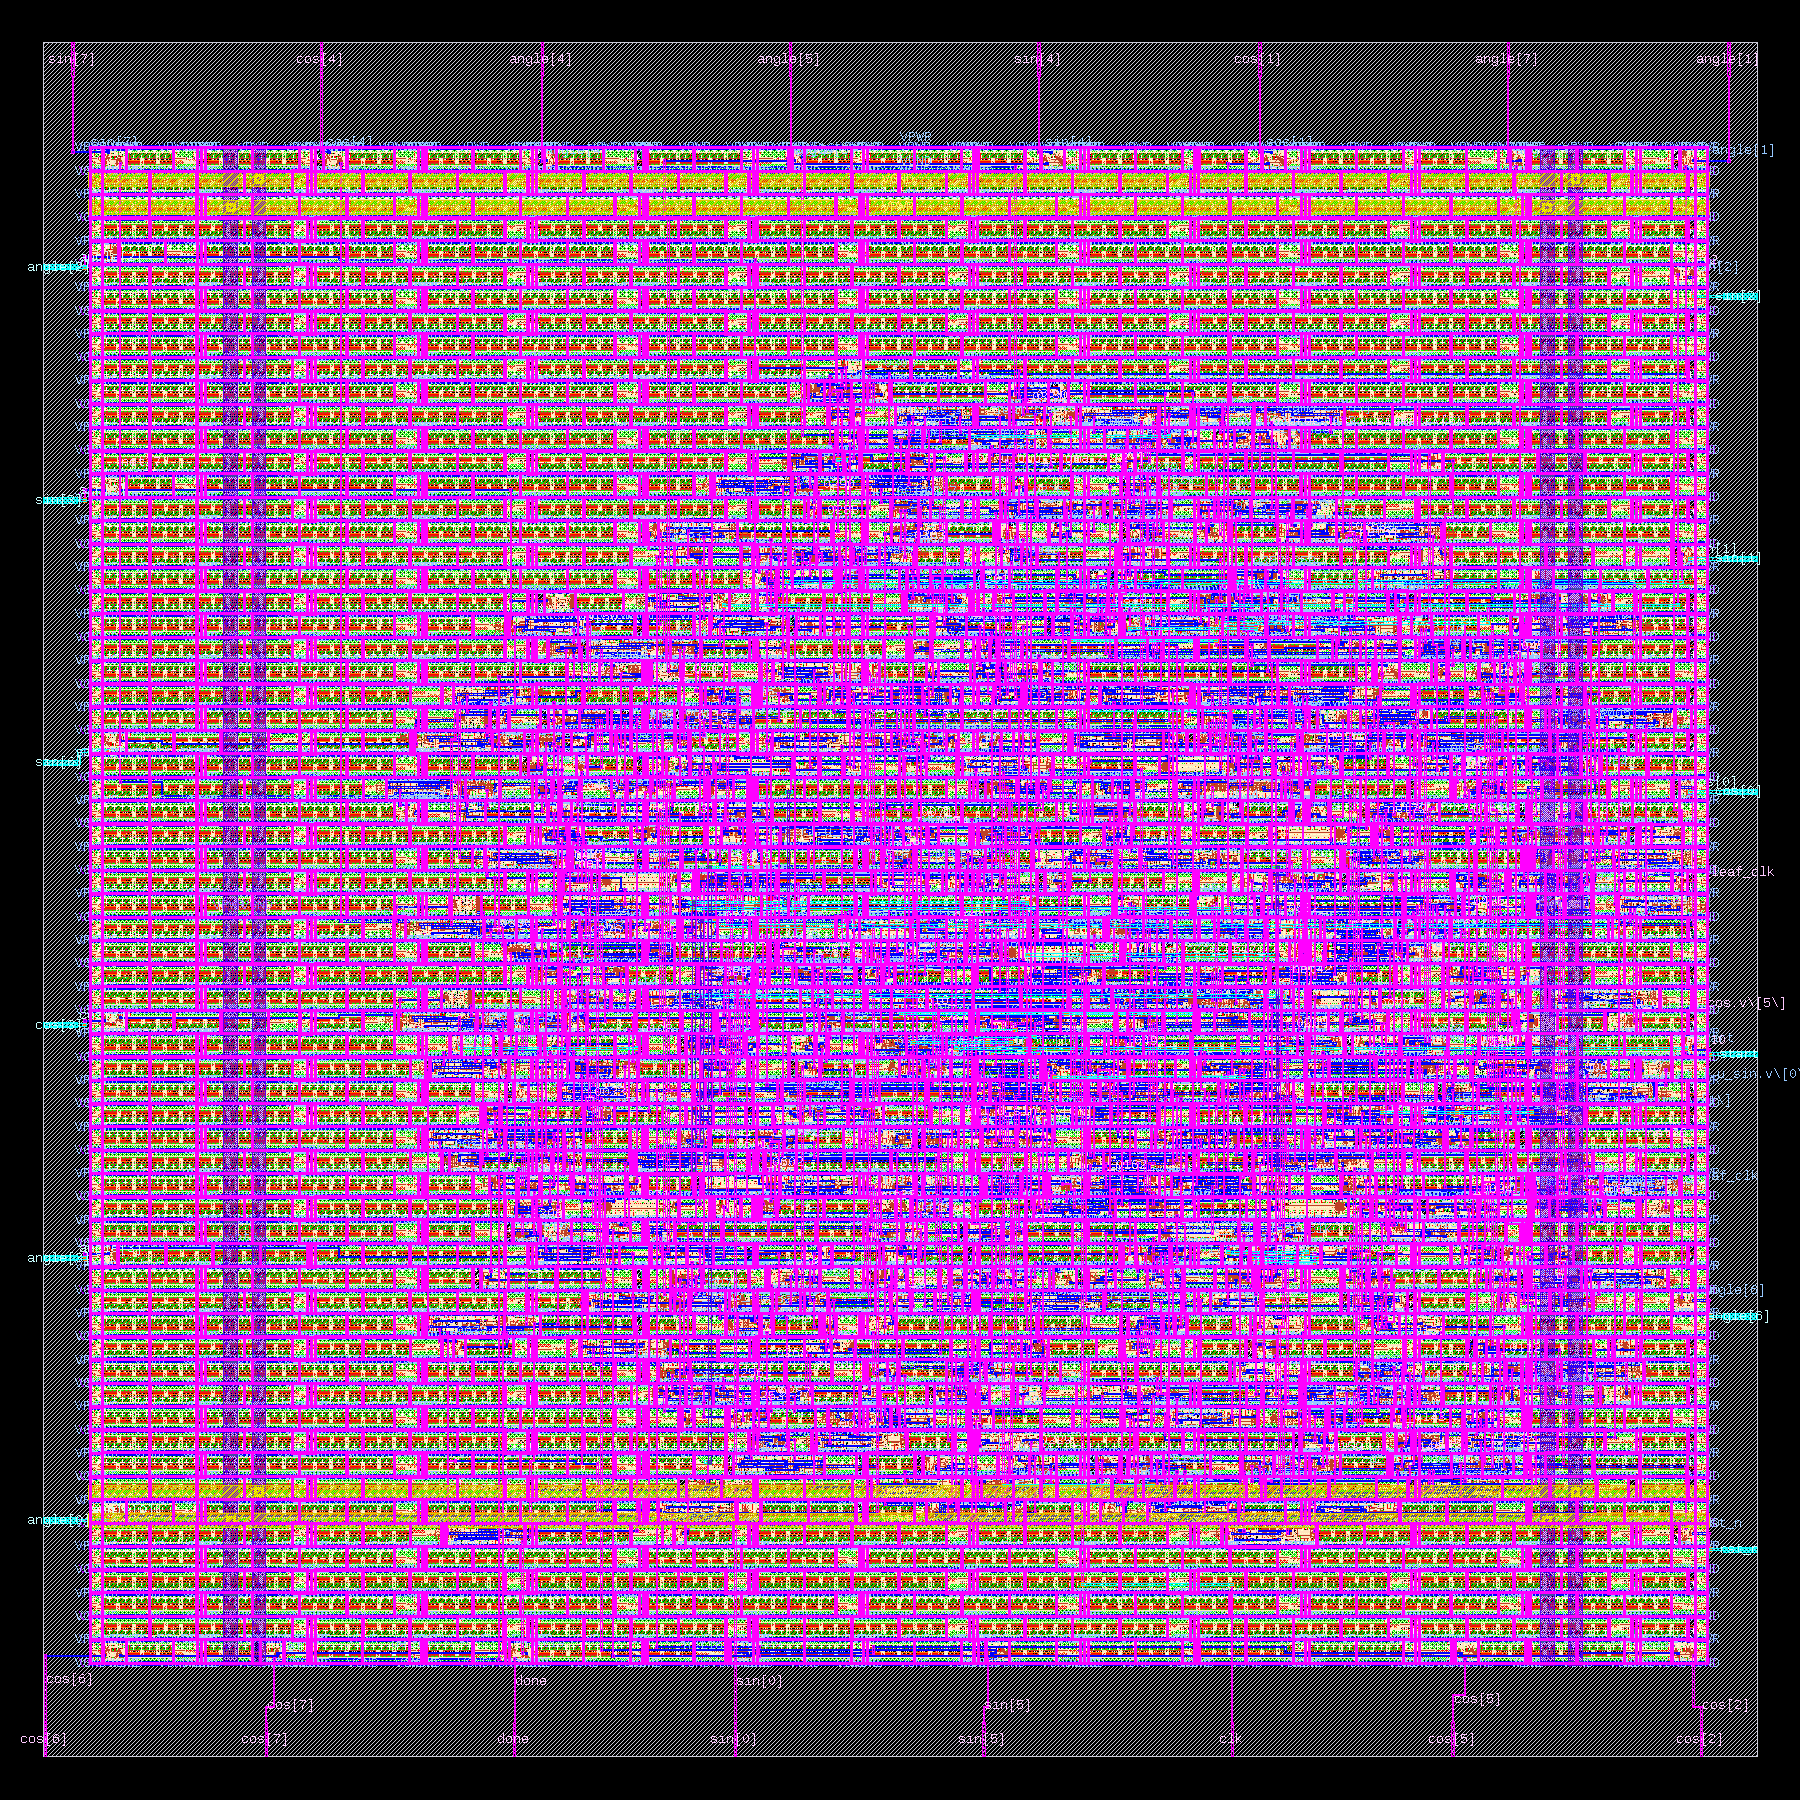
\includegraphics[width=0.72\textwidth]{cordic_gds.png}
\caption{GDS of the core from the kept OpenLane run.}
\label{fig:gds}
\end{figure}

\section{Traceability}

The earlier sections each hold one kind of evidence. This section puts a requirement next to the block that meets it, the file or command that shows it, and the limit of that showing. A claim without a row here is not part of what this report says it has proved.

\subsection{From each requirement to its evidence}
\begin{table}[ht]
\centering
\caption{Requirement, block, evidence, and the limit of that evidence.}
\label{tab:rtm}
\footnotesize
\begin{tabular}{p{0.24\textwidth}p{0.22\textwidth}p{0.24\textwidth}p{0.22\textwidth}}
\toprule
Requirement & Block & Evidence & Limit \\
\midrule
Eight-step rotation, add, subtract, and shift &
\texttt{cordic\_block\_a}, \texttt{cordic\_block\_b}, \texttt{atan\_lut} &
734 cells, 0 multiply cells, 0 memories &
The arctangent \texttt{case} is not its own cell count \\
Charter pins &
\texttt{tt\_um\_cordic} &
\texttt{I05 PIN SHELL PASS} &
The GDS top is \texttt{cordic} \\
Sequential core &
\texttt{dreg}, four states &
66 \texttt{dfrtp\_1} &
The 27--30 hint assumes 8-bit \(x\) and \(y\) \\
Six stored pairs, band \(\pm 4\) &
\texttt{tb\_cordic.v} &
\texttt{I05 RTL TB PASS} &
A difference of 4 still passes \\
Ten angles against true sine and cosine &
\texttt{error\_table.py} &
max \(|\sin|\) 2, max \(|\cos|\) 4 &
These ten codes, not all 256 \\
Clock constraint of the layout &
\texttt{config.tcl} &
\texttt{wns} 0, \texttt{tns} 0 at 10\,ns &
One clock buffer drives 11 loads \\
Layout and GDS &
run \texttt{RUN\_2026.10.03\_09.21.28} &
DRC 0, LVS clean, antenna 0 &
The chip was not fabricated \\
\bottomrule
\end{tabular}
\end{table}

\subsection{What has been shown, and what has not}
On the ten angles in Table~\ref{tab:error}, eight iterations leave at most 2 codes of sine error and 4 codes of cosine error. The cell list shows those iterations as add, subtract, shift, and the eight constants: 734 sky130 cells, 66 flip-flops, no multiplier cell, and no memory. The GDS of the core meets the 10\,ns constraint with routed wires included, Magic DRC is 0, LVS is clean, and the antenna check is 0.

The following are not shown.

\begin{itemize}
  \item The error maximum is the maximum of these ten angles.
  \item A multiplier design was not synthesized, so there is no area saved against a multiplier.
  \item The arctangent constants are inside the 734 cells. Their own cell count was not extracted.
  \item The GDS top is \texttt{cordic}. The pin shell was simulated only.
  \item The run is a local layout. It is not a fabricated chip, and it is not a sign-off.
\end{itemize}

\end{document}
